\documentclass{article}
\usepackage{amsmath}
\usepackage{graphicx}
\usepackage{float}
\usepackage{geometry}
\usepackage{hyperref}
\usepackage{calc}
\usepackage{enumitem}
\usepackage{color}
\usepackage{adjustbox}
\usepackage{xepersian}
\settextfont[
    Scale = 1.3 ,
    BoldFont = *Bd ,
    ItalicFont = *It ,
    Extension = .ttf
]{XB Niloofar}
\AddEnumerateCounter{\alph}{\@alph}{\faalph}

\geometry{
    left=20mm,
    right=20mm,
    top=20mm,
    bottom=20mm,
}


\begin{document}
\begin{titlepage}
    \begin{center}
        \textbf{\Huge{پروژه طراحی سیستم دیجیتال}}\\
        \vspace{1cm}
        
\includegraphics[width=0.3\textwidth]{sharif.jpg}\\
        \vspace{1cm}
        \textbf{ \Large{مزدک تیموریان}}\\
        \vspace{0.4cm}
        \textbf{ \large{401101495}}\\
        \vspace{1cm}
        \textbf{ \Large{دانشکده مهندسی کامپیوتر}}\\
        \vspace{0.4cm}
        \textbf{ \Large{دانشگاه صنعتی شریف}}\\
        \vspace{0.6cm}
        \large{تیر 1403}
    \end{center}
    \thispagestyle{empty}
\end{titlepage}

\section*{طراحی مدار برای مدیریت پارکینگ
(سؤال 8 میانترم)}

\begin{enumerate}[label=\textbf{\alph*)}]
    \item ابتدا ماژولی طراحی میکنیم که نقش ساعت را داشته باشد.
    \begin{figure}[H]
        \centering
        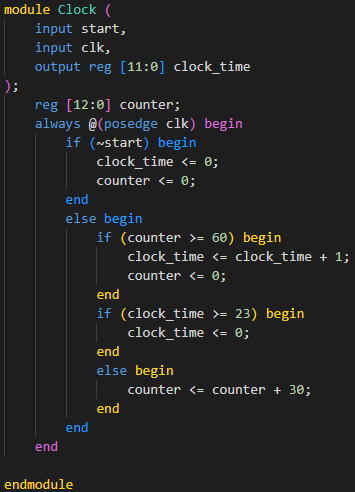
\includegraphics[width=0.7\textwidth]{Clock.png}
    \end{figure}
    همانطور که در شکل بالا مشاهده میکنید این ماژول با ورودی گرفتن سیگنال 
    clk
    و
    start
    شروع به شمارش کرده و به ازای هر 60 چرخه مقدار 
    clock\_time
    را یکی زیاد میکند که نماینده ساعت است و همچنین ساعت بعد از گذر از 23 دوباره 0 میشود.
    (روز بعد)

    حال از این ماژول در ماژول اصلی استفاده میکنیم.

    \begin{figure}[H]
        \centering
        \begin{minipage}{0.4\textwidth}
            \centering
            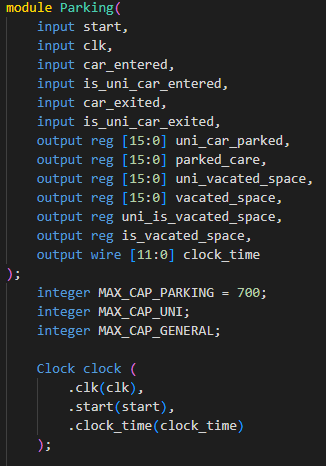
\includegraphics[width=\textwidth]{Parking1.png}
        \end{minipage}\hfill
        \begin{minipage}{0.5\textwidth}
            \centering
            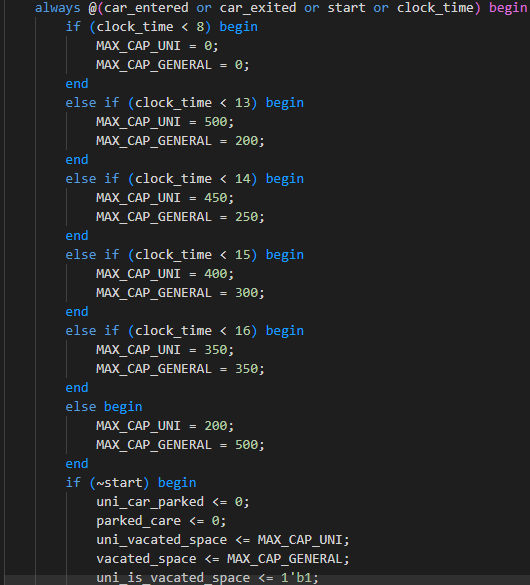
\includegraphics[width=\textwidth]{Parking2.png}
        \end{minipage}
    \end{figure}
نحوه کار پارکینگ با توجه به ساعت بصورت زیر است
\begin{itemize}
    \item از ساعت 0 تا 8 هیچ ماشینی نمیتواند وارد شود و صرفاً ماشین‌هایی که از قبل داخل پارکینگ بودند
    میتوانند خارج شوند.
    \item از ساعت 8 تا 13 ظرفیت دانشگاه برابر با 500 و ظرفیت آزاد 200 ماشین است.
    \item از ساعت 13 تا 14 ظرفیت دانشگاه و آزاد به ترتیب برابر با 450 و 250 است.
    \item از ساعت 14 تا 15 ظرفیت دانشگاه و آزاد به ترتیب برابر با 400 و 300 است.
    \item از ساعت 15 تا 16 ظرفیت دانشگاه و آزاد به ترتیب برابر با 350 و 350 است.
    \item از ساعت 16 تا 24 ظرفیت دانشگاه و آزاد به ترتیب برابر با 200 و 500 است.
\end{itemize}
توجه کنید در صورتی که بعد از تغییر ساعت تعداد ماشین‌های یک گروه بیشتر از ظرفیت آنها درون پارکینگ شوند این مقدار بیش از ظرفیت با عددی منفی نمایش داده شده 
و تنها درصورتی ماشین جدید از آن گروه میتواند وارد پارکینگ شود که تمامی ماشین‌های مضاف بر
ظرفیت از پارکینگ خارج شوند.

\newpage
حال در ادامه منطق ورود و خروج پیاده‌سازی شده است.
\begin{figure}[H]
    \centering
    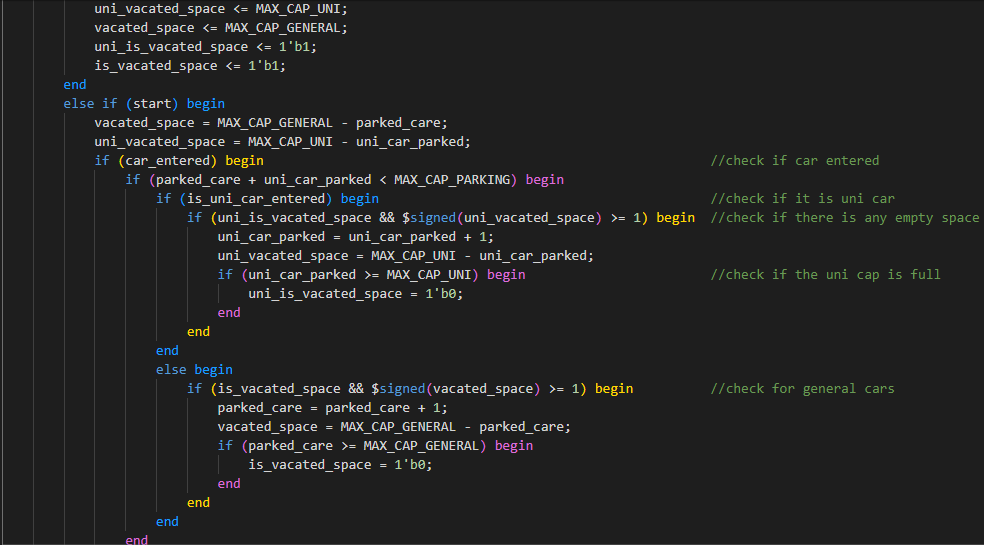
\includegraphics[width=\textwidth]{Parking3.png}
\end{figure}
\begin{figure}[H]
    \centering
    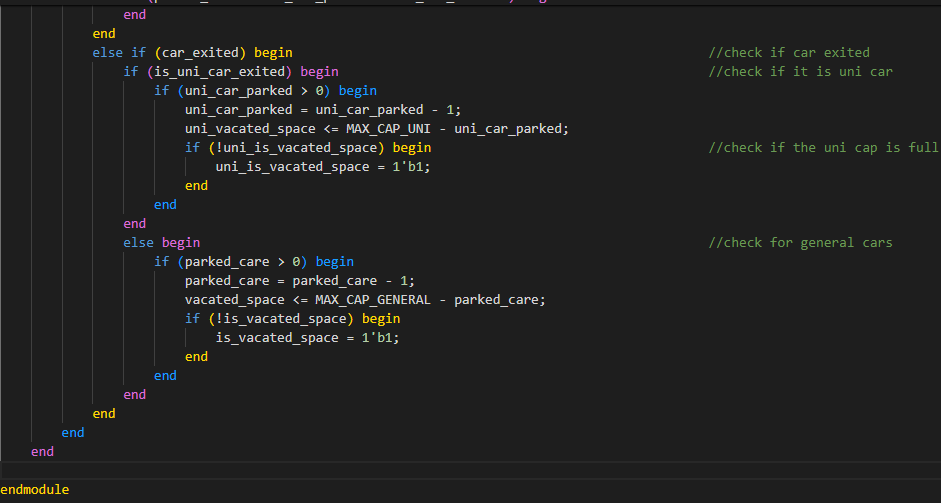
\includegraphics[width=\textwidth]{Parking4.png}
\end{figure}

ماژول تست طراحی شده برای ماژول بالا نیز بصورت زیر است.

\begin{figure}[H]
    \centering
    \begin{minipage}{0.45\textwidth}
        \centering
        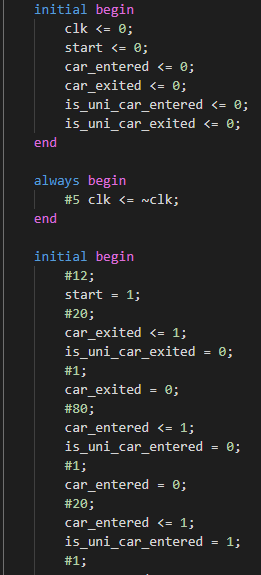
\includegraphics[width=\textwidth]{Test1.png}
    \end{minipage}\hfill
    \begin{minipage}{0.45\textwidth}
        \centering
        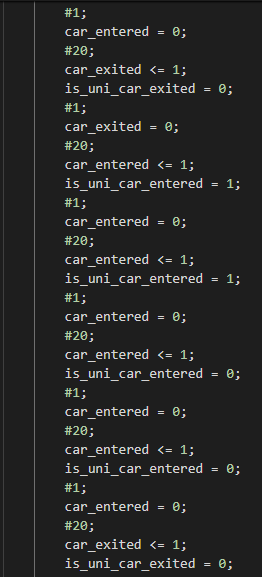
\includegraphics[width=\textwidth]{Test2.png}
    \end{minipage}
\end{figure}

\begin{figure}[H]
    \centering
    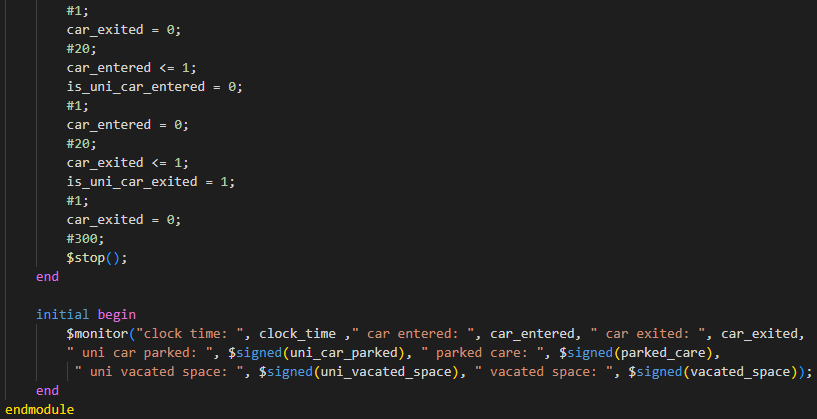
\includegraphics[width=\textwidth]{Test3.png}
\end{figure}
نحوه عملکرد ماژول تست را میتوانید در شکل‌های زیر مشاهده کنید.
(توجه کنید که برای آزمایش پر شدن پارکینگ تعداد ورود و خروج ماشین‌ها 100 تایی
گذاشته شده‌اند.)

\begin{figure}[H]
    \centering
    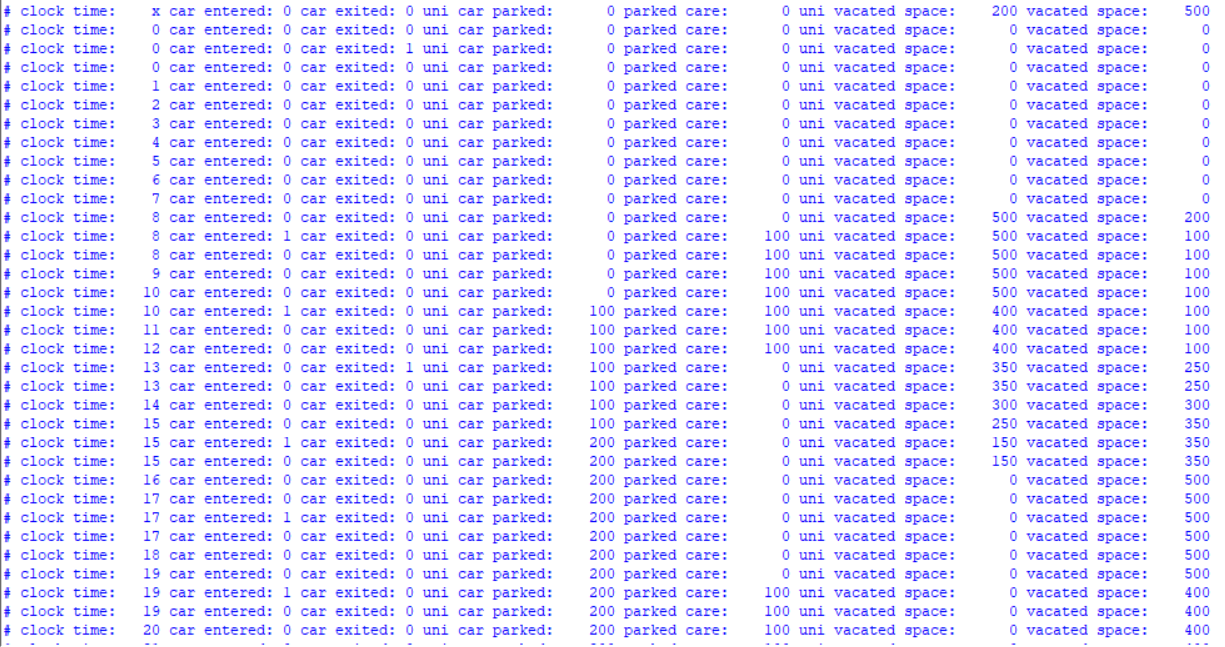
\includegraphics[width=\textwidth]{Results1.png}
\end{figure}
\begin{figure}[H]
    \centering
    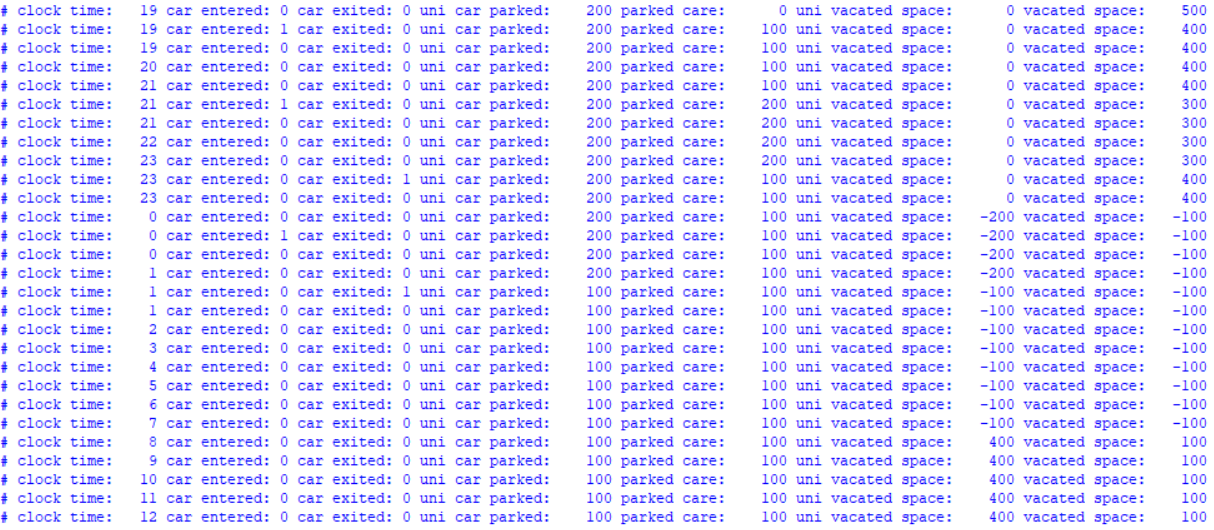
\includegraphics[width=\textwidth]{Results2.png}
\end{figure}

در شکل زیر نیز نحوه عملکرد ماژول در حالت معمولی را میتوانید مشاهده کنید.
\begin{figure}[H]
    \centering
    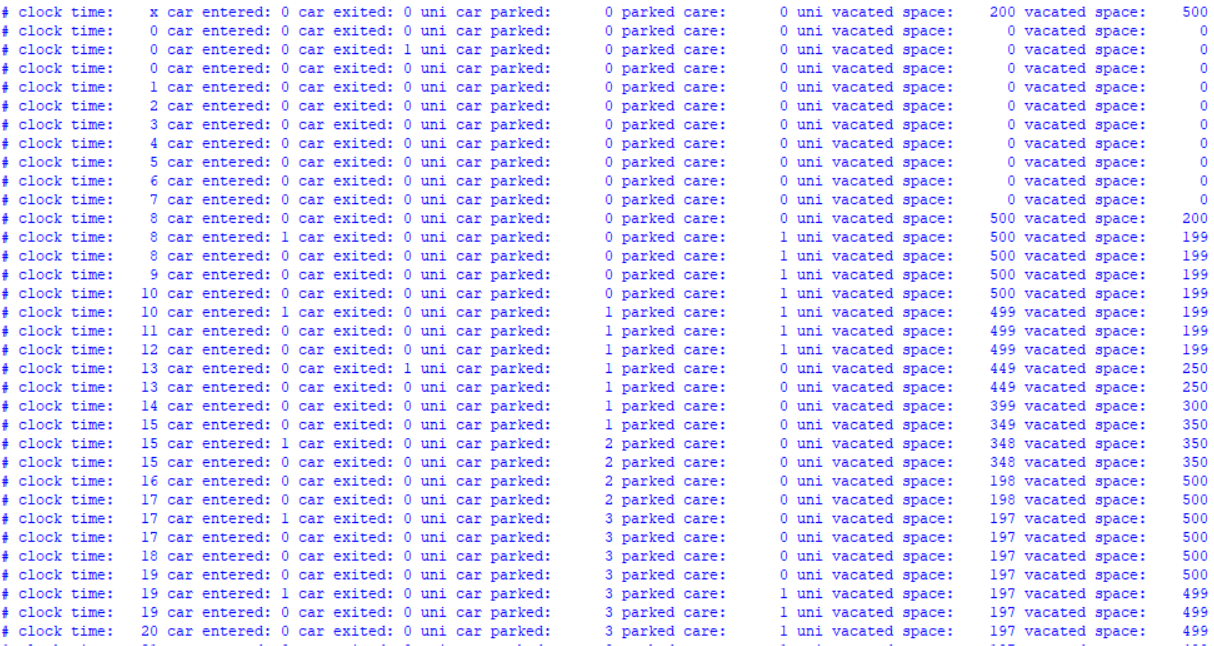
\includegraphics[width=\textwidth]{Results3.png}
\end{figure}

\item در این قسمت با استفاده از نرم‌افزار 
Quartus
مدار را سنتز میکنیم.
که نتایج آن در شکل‌های زیر قابل مشاهده است.
\begin{figure}[H]
    \centering
    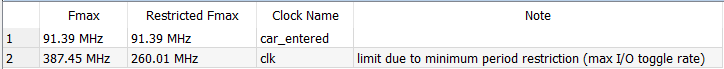
\includegraphics[width=\textwidth]{Fmax.png}
\end{figure}
در شکل بالا بیشترین مقدار فرکانس مدار قابل مشاهده است 
(\begin{large}
    $387.45M_{Hz}$
\end{large}
در حالت بدون محدودیت 
I/O
و 
\begin{large}
    $260.01M_{Hz}$
\end{large}
با محدودیت 
I/O )

عامل محدود کننده فرکانس تأخیر مسیر بحرانی است.
\begin{figure}[H]
    \centering
    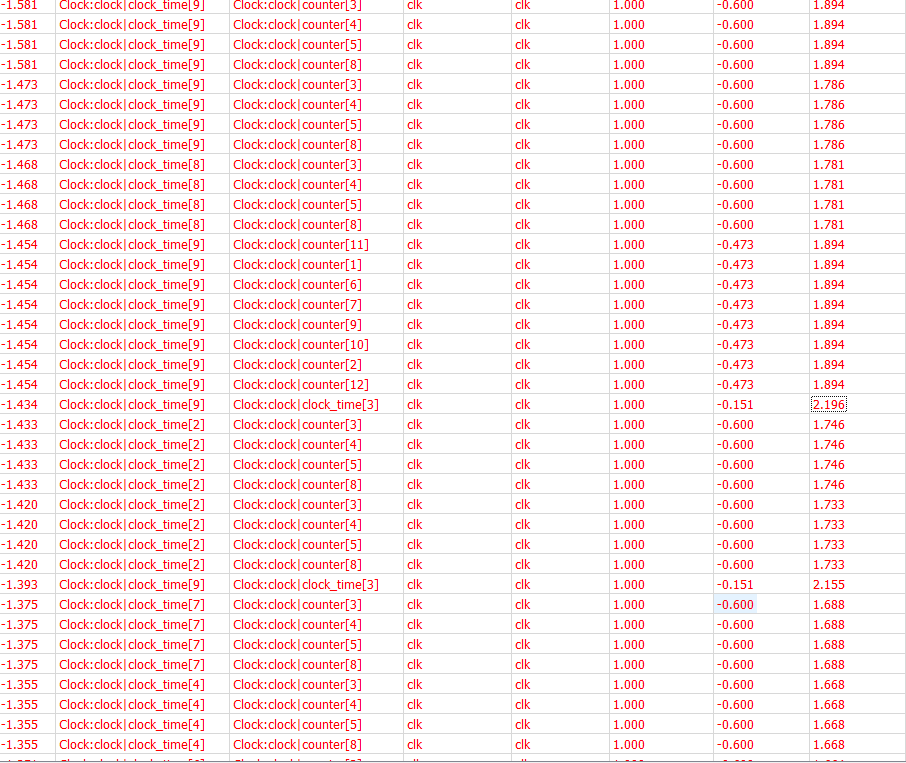
\includegraphics[width=\textwidth]{Delay.png}
\end{figure}

شکل بالا نیز که نشان دهنده مسیرهای با بیشترین تأخیر است با معکوس کردن بیشترین تأخیر آن با تقریب خوبی
به فرکانس نشان داده شده میرسیم.

\begin{large}
    $$1.894 + 0.473 = 2.367 = T \Rightarrow \frac{1}{T} \approx 0.422 \approx 0.38745 \pm 0.050$$
\end{large}
\end{enumerate}

\end{document}